%%%%%%%%%%%%%%%%%%%%%%%%%%%%%%%%%%%%%%%%%%%%%%%%%%%%%%%%%%%%%%%
%%% Cap\'itulo: SCCP %%%
%%%%%%%%%%%%%%%%%%%%%%%%%%%%%%%%%%%%%%%%%%%%%%%%%%%%%%%%%%%%%%%
\chapter{SCCP}
\label{cap3.sccp}      

... introducci\'on al capitulo

%%% Secci\'on: Modalidades espaciales y epist\'emicas en sistemas de restricciones %%%

\section{Modalidades espaciales y epist\'emicas en sistemas de restricciones}
\label{mod.cap3}

Concurrent constraint programming (\textbf{ccp}) es un modelo computacional en el cual agentes (procesos, usuarios, etc) interact\'uan sobre un almac\'en de informaci\'on compartido, el cual puede contener informaci\'on parcial. La notaci\'on cl\'asica de las operaciones \textit{read} and \textit{write} es reemplazada por la notaci\'on \textit{ask} and \textit{tell}. La operaci\'on \textit{ask} intenta inferir si es posible obtener informaci\'on de los procesos, mientras que la operaci\'on \textit{tell} agrega informaci\'on parcial al almac\'en de los procesos.

Las caracter\'isticas de \textbf{ccp} lo hacen un formalismo declarativo en cual permite la implementaci\'on de diferentes sistemas reactivos. En este area \textbf{ccp} se ha extendido para modelar diferentes tipos de concurrencia y abordar problemas que surgen en la modelaci\'on de sistemas reactivos, dichas extensiones incluyen, no-determinismo, movilidad y comportamiento sincronizado. La extension mas resiente agrega modalidades epist\'emica y espacial, que permiten modelar comportamiento distribuido, el cual no rea posible con las extensiones antes mencionadas.

Sin embargo, esta extension requiere de algunas definiciones particulares sobre los conceptos usados en \textbf{ccp}.

% Subsecci\'on: Sistema de restricciones simple
\subsection{Sistema de Restricciones Simple}
\label{srs.cap3}

El modelo \textbf{ccp} es param\'etrico en un sistema de restricciones (\textit{cs}). Esto significa que los par\'ametros del proceso son restricciones que pertenecen a alguno de las teor\'ias de primer orden utilizadas en el sistema de restricciones. El \textit{cs} es la estructura que especifica las interdependencias de la informaci\'on usada en el almac\'en compartido. 

De acuerdo con~\cite{DEBOER199537} las restricciones del sistema se pueden ver como un entramado algebraico completo. Este entramado es provisto del ordenamiento $\sqsubseteq$, definido formalmente como:

\theoremstyle{definition}
\begin{definition}{Sistema de restricciones.}
Un sistema de restricciones es un entramado algebraico completo $C = (Con, Con_0, \sqsubseteq, \sqcup, true, false)$ donde $Con$ es el conjunto de restricciones, $Con_0$ es el conjunto de elementos compactos de $Con$ y esta ordenado con respecto a $\sqsubseteq$, $\sqcup$ es la operaci\'on del l\'imite inferior definido en subconjuntos, y $true, false$ son son el menor y mayor elemento de $Con$.
\end{definition}

% Subsecci\'on: Sistema espacial de restricciones 
\subsection{Sistema Espacial de Restricciones}
\label{ser.cap3}

Para \textbf{sccp} es necesario definir un sistema espacial de restricciones, el cual es una extensi\'on de la definici\'on de un sistema de restricciones. El objetivo es modelar un sistema distribuido de multiples agentes en el que cada agente tiene su propio espacio de computaci\'on. Esto se obtiene agregando la noci\'on de espacio para un agente, denotado por una funci\'on $s_i(c)$, que significa que una restricci\'on $c$ esta contenida en el espacio del agente $i$. Formalmente, un \textit{sistema espacial de restricciones de n agentes} se define como sigue:

\theoremstyle{definition}
\begin{definition}{Sistema espacial de restricciones de n agentes (n-scs).}
Un sistema espacial de restricciones de n agentes (n-scs) es un sistema de restricciones \textbf{C} provisto con n mapas ($s_1, \mathellipsis,s_n$) sobre su conjunto de restricciones $Con$.  Cada mapa $s_i: Con \rightarrow Con$ debe satisfacer las siguientes propiedades:
\begin{equation} \label{n-scs.eq1}	
s_i(true)=true 
\end{equation}
\begin{equation} \label{n-scs.eq2}
s_i(c\sqcup d)=c\sqcup d
\end{equation}
\begin{equation} \label{n-scs.eq3}
c \sqsubseteq d \Rightarrow s_i(c) \sqsubseteq s_i(d)
\end{equation}
\end{definition}

Esto muestra que cada $s_i$ es el espacio de funci\'on del agente $i$. Formalmente un c-scs puede ser denotado $C = (Con, Con_0, \sqsubseteq, \sqcup, true, false, s_1, \mathellipsis, s_n)$. 

La ecuaci\'on~\ref{n-scs.eq1} expone que tener un almac\'en local sin informaci\'on es igual a no tener informaci\'on globalmente.  La ecuaci\'on~\ref{n-scs.eq2} hace posible unir informaci\'on diferente que esta en el mismo espacio, finalmente la ecuaci\'on~\ref{n-scs.eq3} significa que si $c$ puede ser derivado de $d$, entonces cualquier agente puede derivar esto en su propio espacio.

En un modelo n-scs, nada previene que haya informaci\'on inconsistente entre agentes. Esto es conocido como \textit{confinamiento de inconsistencias}.

Existe otra propiedad en los sistemas espaciales de restricciones llamada: \textit{preservaci\'on de distinci\'on}. Esta propiedad se refiere al hecho de que en algunos casos puede suceder $s_i(c)=s_i(d)$ con $c\neq d$. Esto puede ser interpretado como la imposibilidad del agente $i$ de distinguir entre $c$ y $d$. Sin embargo, en algunas aplicaciones esta propiedad puede ser necesaria.

Por ultimo, se debe introducir el concepto de \textit{informaci\'on compartida} e \textit{informaci\'on global}. Informalmente, \textit{informaci\'on compartida} sobre un grupo \textbf{G} se refiere a la informaci\'on que es compartida entre agentes de dicho grupo. Mientras que \textit{informaci\'on global} se refiere al hecho de que informaci\'on $c$ esta presente en cada espacio anidado.

% Subsecci\'on: Sistema epist\'emico de restricciones 
\subsection{Sistema Epist\'emico de Restricciones}
\label{sepr.cap3}

Mientras que la informaci\'on en n-scs representa lo que puede ser entendido como creencias, el objetivo de un sistema epist\'emico de restricciones es modelar conocimiento. Por lo tanto, cada informaci\'on $c$ es un hecho que un agente $i$ conoce. Este hecho es representado por la misma estructura de n-scs, es decir, $s_i(c)$. Desde un punto de vista epist\'emico, el concepto de consistencia del espacio no se mantiene, puesto que es imposible para un agente tener conocimiento inconsistente. En otras palabras, cada pieza de conocimiento de un agente, debe ser cierta, y por esta raz\'on no aplica el concepto de consistencia del espacio.

\theoremstyle{definition}
\begin{definition}{Sistema epist\'emico de restricciones de n agentes (n-ecs).}
Un sistema epist\'emico de restricciones de n agentes (n-ecs) es un sistema n-scs cuyas funciones de espacio $s_1, \mathellipsis, s_n$ tambi\'en son operadores de clausura, y ademas de las propiedades~\ref{n-scs.eq1},~\ref{n-scs.eq2} y~\ref{n-scs.eq3}, satisfacen:
\begin{equation} \label{n-ecs.eq1}
c \sqsubseteq s_i(c)
\end{equation}
\begin{equation} \label{n-ecs.eq2}
s_i(s_i(c))=s_i(c)
\end{equation}
\end{definition}

La propiedad~\ref{n-ecs.eq1} expone que si un agente conoce una pieza de informaci\'on, entonces esa informaci\'on debe ser cierta. Esto significa que $s_i(c)$ contiene por lo menos tanta informaci\'on como $c$. De otro lado, la segunda propiedad se refiere al hecho de que un agente es consiente de la informaci\'on que conoce. 

%%% Secci\'on: Espacios y conocimiento en procesos %%%
\section{Espacios y conocimiento en procesos}
\label{ecp.sccp}

Ahora se presentan dos variantes del modelo \textbf{ccp}, llamados programaci\'on espacial concurrente de restricciones y programaci\'on epist\'emica concurrente de restricciones (\textbf{sccp} y \textbf{eccp}, por sus siglas en ingles). El primero se refiere a un c\'alculo que solo permite ejecutar procesos dentro del espacio de un agente, posiblemente anidado, mientras que el segundo extiende este comportamiento a la interacci\'on entre agentes solicitando y procesando conocimiento dentro de la distribuci\'on espacial de informaci\'on. Cada extensi\'on utiliza un scs y ecs respectivamente.

% Subsecci\'on: Sintaxis de procesos
\subsection{Sintaxis de procesos}
\label{spr.cap3}

Ahora se presenta la sintaxis para los procesos \textbf{sccp} y \textbf{eccp}.

\theoremstyle{definition}
\begin{definition}{Sintaxis general.}
Los t\'erminos de ambos lenguajes es presentada por la siguiente sintaxis:
%\begin{equation} \label{e-sccp.eq1}
%P,Q, \mathellipsis ::=\textbf{0} | \textbf{tell(c)} | \textbf{ask(c)} \rightarrow \textbf{P} | P\|Q | [P]_i
%\end{equation}
\[P,Q, \mathellipsis ::=\textbf{0} | \textbf{tell(c)} | \textbf{ask(c)} \rightarrow \textbf{P} | P\|Q | [P]_i\]
\end{definition}

Para \textbf{sccp} el sistema de restricci\'on es n-scs, y para \textbf{eccp} es n-ecs. A continuaci\'on se describe brevemente el significado de cada operador:

\begin{itemize}
\item $\textbf{0}$ representa la inactividad de un proceso, es decir, que no hace nada.
\item El proceso $\textbf{tell(c)}$ agrega informaci\'on al almac\'en.
\item El proceso $\textbf{ask(c)} \rightarrow \textbf{P}$ verifica si la restricci\'on $c$ es una implicaci\'on del almac\'en actual y despu\'es ejecuta el proceso $\textbf{P}$.
\item El proceso $P\|Q$ es para la ejecuci\'on en paralelo de procesos.
\item El proceso $[P]_i$ ejecuta $P$ dentro del espacio de computaci\'on del agente $i$.
\end{itemize}

%%% Secci\'on: Sem\'antica operacional estructurada para espacios y conocimiento en procesos %%%

\section{Sem\'antica operacional estructurada}
\label{soe.esi}

La semantica operacional estructurada (SOS) 
La reducci\'on es hecha por medio de configuraciones de la forma $\langle P,d\rangle \rightarrow \langle P',d'\rangle$, donde $P,P'$ denotan procesos, y $c,c'$ denotan el almac\'en de los procesos. Las reglas comunes entre ambos lenguajes se expresan a continuaci\'on. El simbolo $\gamma$ representa un grupo de configuraciones.

\begin{figure*}[pthb]
  \centering
  \begin{minipage}[c]{0.8\textwidth}%
	\begin{center}
  %  \input{images/sos.png}
    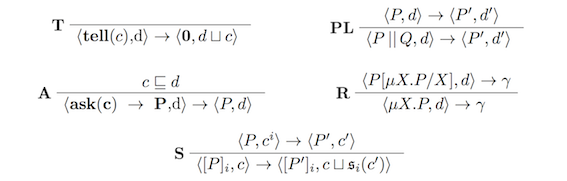
\includegraphics[width=12cm]{images/sos.png}
  \end{center}
\end{minipage}
  \caption{SOS para \textbf{sccp} y \textbf{eccp}}
  \label{fig.sos}
\end{figure*}

Las reglas mostradas en la figura~\ref{fig.sos} confirman lo explicado hasta este punto del trabajo. Por ejemplo, en la regla \textbf{T} la restricci\'on $c$ se agrega al almac\'en y luego el proceso se reduce a \textbf{0}. En el caso de la regla \textbf{A}, si la guarda $c$ es implicaci\'on del almac\'en, entonces el proceso se reduce y se ejecuta $P$. \textbf{PL} muestra que se puede ejecutar $P$ o $Q$. Por ultimo, el proceso que es ejecutado dentro del espacio de un agente, la restricci\'on se agrega dentro del espacio de dicho agente. Estas reglas funcionan para las reducciones comunes en \textbf{sccp} y \textbf{eccp}. Sin embargo, en \textbf{eccp} hay una regla adicional la cual permite modelar el hecho de que la informaci\'on conocida por un agente $i$ se convierte en un hecho. Esta regla se define a continuaci\'on. 

\begin{figure*}[pthb]
  \centering
  \begin{minipage}[c]{0.8\textwidth}%
	\begin{center}
  %  \input{images/sos.png}
    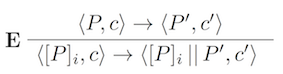
\includegraphics[width=6cm]{images/eccp_sos.png}
  \end{center}
\end{minipage}
%  \caption{SOS para \textbf{sccp} y \textbf{eccp}}
  \label{fig2.sos}
\end{figure*}

Despu\'es de definir el lenguaje que se va a usar, se procede a definir la especificaci\'on formal para dicho lenguaje. 













